%
% ========================================================================
%
%  	
%
%   Authors: Shijie Shu 
%   Created: Jan, 2016.
%
% ========================================================================
% ----------------------------------
%  Class and Packages
% ----------------------------------

\documentclass[portait,custom]{sciposter}
%\documentclass[12pt]{report}
%\documentclass[landscape,custom]{sciposter}

% ----------------------------------
%  Customization and Macros
% ----------------------------------

\usepackage{local}

%\usepackage{hyperref}
%\hypersetup{colorlinks=true,citecolor=black,filecolor=black,linkcolor=black,urlcolor=black,breaklinks=true}
%\usepackage{columns}
\usepackage{supertabular}
\usepackage{rotating,multirow}
\usepackage[multidot]{grffile}
\usepackage{dcolumn}
\newcolumntype{s}{D{.}{.}{1.2}}
\usepackage{natbib}
\bibpunct{(}{)}{;}{a}{,}{,~}
%\usepackage[comma,sort]{natbib}
%\bibliographystyle{plainnat}

\usepackage{comment}

\usepackage{sectionbox}

\definecolor{CCSIGreen}{rgb}{0.16,0.46,0.29} % Hex #29754b
\definecolor{CCSILightGreen}{rgb}{0.90,1.0,0.80}

% ========================================================================
\leftlogo{\hspace*{+0.00in}
           \raisebox{-270pt}{
\includegraphics[height=2.50in,trim=1cm 1cm 1cm 1cm,clip=true]{logos/ACME_Logo.pdf}}%
           \raisebox{-280pt}{
\includegraphics[height=2.60in]{logos/ORNL_logo}}%
           \hspace*{75pt}%
           %\raisebox{-300pt}{
\includegraphics[height=2.40in]{logos/CCSI_logo_FMH.pdf}}%
           %\raisebox{-120pt}{
\includegraphics[height=1.90in]{logos/LBNL_logo.png}}%
}
\rightlogo{\hspace*{-7.50in} 
           %\hspace*{-1.0in}
           %\raisebox{-130pt}{
\includegraphics[height=2.00in]{logos/USFS_Logo.png}}%
           %\hspace*{75pt}%
           %\raisebox{-130pt}{
\includegraphics[height=2.00in]{logos/intel_logo.png}}%
            %\raisebox{-270pt}{
\includegraphics[height=1.95in]{logos/ORNL_logo}}%
            %\raisebox{-180pt}{
\includegraphics[height=1.80in]{logos/CCSI_logo_FMH.pdf}}%
%            \raisebox{-250pt}{
\includegraphics[height=2.50in]{logos/CCSI_Text_Logo_transparent.png}}%
            %\raisebox{-260pt}{
\includegraphics[height=1.80in]{logos/LBNL_logo.png}}%
           %\raisebox{-350pt}{
\includegraphics[height=3.0in]{logos/ACME_Logo.pdf}}%
           % \hspace*{25pt}%
           %\raisebox{-375pt}{
\includegraphics[height=2.50in]{logos/ess_logo_white.pdf}}%
           %\hspace*{25pt}%
           %\raisebox{-355pt}{
\includegraphics[height=1.80in]{logos/USFS_Logo.pdf}}%
}

\newcommand{\VERYHUGE}{\fontsize{105}{200.0}\selectfont}

%\title{\VERYHUGE Forecasting Pan-Tropical Ecological Impacts of the \\ \medskip 2015 El Ni\~{n}o Southern Oscillation (ENSO)}
\title{\VERYHUGE Estimating Potential Damping of Cryoturbation on Permafrost Carbon Emissions Using a Perturbed Parameters Approach in a Land Surface Model}

\author{
  Shijie~Shu$^\textnormal{1}$,
  Umakant~Mishra$^\textnormal{2}$,
  James~T.~Randerson$^\textnormal{3}$,
  Yujie~He$^\textnormal{3}$, \\
  Charles~D.~Koven$^\textnormal{4}$, 
  Forrest~M.~Hoffman$^\textnormal{5}$,
  and
  Atul~K.~Jain$^\textnormal{1}$
  }

% institute name
\institute{
  $^\textnormal{1}$Department~of~Atmospheric~Science,~University~of~Illinois~(UIUC),
  $^\textnormal{2}$Argonne~National~Laboratory~(ANL),\\
  $^\textnormal{3}$University~of~California~Irvine~(UCI),
  $^\textnormal{4}$Lawrence~Berkeley~National~Laboratory~(LBNL),
  and
  $^\textnormal{5}$Oak~Ridge~National~Laboratory~(ORNL)
  %$^\textnormal{3}$Intel~Corp.
  %$^\textnormal{4}$USDA~Forest~Service
}


% ========================================================================
\setmargins[10cm]

\begin{document}

\conference{American Geophysical Union (AGU) 2016 Fall Meeting (December 12--16, 2016), Moscone Center, San Francisco, CA, USA \hfill Department of Atmospheric Sciences, University of Illinois at Urbana-Champaign.}

\maketitle

% For the SciDAC3 PI Meeting, we are forbidden to use any DOE logos!
%\includegraphics[height=1.25in]{logos/ANL_logo}\hfill\includegraphics[height=1.25in]{logos/LLNL_logo}\hfill\includegraphics[height=1.25in]{logos/LANL_logo}\hfill\includegraphics[height=1.25in]{logos/NCAR_logo}\hfill
\includegraphics[height=1.25in]{logos/ORNL_logo}\hfill\includegraphics[height=1.25in]{logos/PNNL_logo}\hfill\includegraphics[height=1.25in]{logos/SNL_logo}

\vspace{-1.0in}

\begin{multicols*}{4}

%%%%%%%%%%%%%%%%%%%%%%%%%%%%%%%%%%%%%%%%%%%%%%%%%%%%%%%%%%%%%%%%%%%%%%%%%%%%%%%
%\section*{Introduction}
\section*{Introduction}
%%%%%%%%%%%%%%%%%%%%%%%%%%%%%%%%%%%%%%%%%%%%%%%%%%%%%%%%%%%%%%%%%%%%%%%%%%%%%%%

%The El Ni\~{n}o Southern Oscillation (ENSO) is an irregular periodic
%climate fluctuation, occurring every eight to 12 years, that is driven
%by variations in sea surface temperatures (SSTs) over the tropical
%eastern Pacific Ocean and extending westward across the equatorial
%Pacific. The warming phase is called El Ni\~{n}o and the cooling phase
%is called La Ni\~{n}a. This dominant ocean cycle, linked with the
%Walker Circulation, affects ocean turnover and nutrient availability,
%as well as temperatures and precipitation globally. El Ni\~{n}o also
%has strong effects on the global carbon cycle seasonally because,
%although weakened ocean circulation reduces marine carbon outflow,
%terrestrial emissions more than compensate for this reduction. Strong
%drying conditions in the Asia-Pacific region and western South America
%during El Ni\~{n}o lead to reduced ecosystem productivity and increased
%mortality and fire risk, which are responsible for the increased source
%of carbon to the atmosphere.
Permafrost soils in the northern high latitudes (NHLs) contain about half of the world's total soil organic carbon (SOC), which has a potential to be a large carbon source as a consequence of anticipated climate changes. Few studies addressed the role of cryoturbation on future soil organic carbon storage in NHLs. Here we coupled a land surface model, Integrated Science and Assessment Model, with one dimensional soil biogeochemistry (ISAM-1DSB) to examine how the changes in cryoturbation due to changes in the thermal and hydrological regime will affect the NHL permafrost carbon storage under the IPCC RCP8.5 climate scenario.

%%%%%%%%%%%%%%%%%%%%%%%%%%%%%%%%%%%%%%%%%%%%%%%%%%%%%%%%%%%%%%%%%%%%%%%%%%%%%%
\section*{Rationale}
%%%%%%%%%%%%%%%%%%%%%%%%%%%%%%%%%%%%%%%%%%%%%%%%%%%%%%%%%%%%%%%%%%%%%%%%%%%%%%

\begin{itemize}
  \item Deepening of the active layer under climate warming in permafrost regions exposes a substantial amount of deep soil carbon to the open air, enhancing microbial decomposition of soil organic carbon hence cause a positive permafrost carbon climate feedback to accelerate the warming trend.

  \item Cryoturbation process, that is the displacement of soil during seasonal and/or diurnal freezing and thawing, may damping this feedback (Pinget al., 2015) since:
  \begin{itemize}

    \item The elongated duration of freezing/thawing under warming may strengthen the frost heave activities, bringing more soil organic carbon (SOC) downward to be stabilized.

    \item The increased active layer thickness (ALT) cause more SOC being cryoturbated.

  \end{itemize}
\end{itemize}

%%%%%%%%%%%%%%%%%%%%%%%%%%%%%%%%%%%%%%%%%%%%%%%%%%%%%%%%%%%%%%%%%%%%%%%%%%%%%%
\section*{Model Description}
%%%%%%%%%%%%%%%%%%%%%%%%%%%%%%%%%%%%%%%%%%%%%%%%%%%%%%%%%%%%%%%%%%%%%%%%%%%%%%

\subsection*{ISAM-1DSOC}

\begin{itemize}

 \item ISAM land surface model contains fully coupled biogeophysical and biogeochemical cycles. Recent advancements of the model on representing permafrost hydrology and carbon cycle include:
 \begin{itemize}
   \item Snow compaction, depth hoar formation and SOC thermal insulation processes to accurately account the soil thermal status and permafrost table depth. (Barman and Jain, 2016)
   \item Vertically resolved soil biogeochemistry to account for the vertical movement of SOC and the SOC profile under different long-timescale forces (bioturbation, cryoturbation and sediment deposition) (Shu et al., 2015)
   \item Hydraulic impedance of ice and the perched water table to refine the model performance on arctic hydrology and the seasonal wet soil and wetland. (Swenson et al., 2012)
   \item Aqueous and gaseous $CH_4$ and $O_2$ diffusion, $CH_4$ production, oxidation and ebullition in the wet soil to consider the preservation of SOC through preventing the aerobic decomposition under the prevailing seasonal anoxic environment in permafrost region. (Shu et al., 2017, in prep)
 \end{itemize}

\begin{figure}
 \centering
  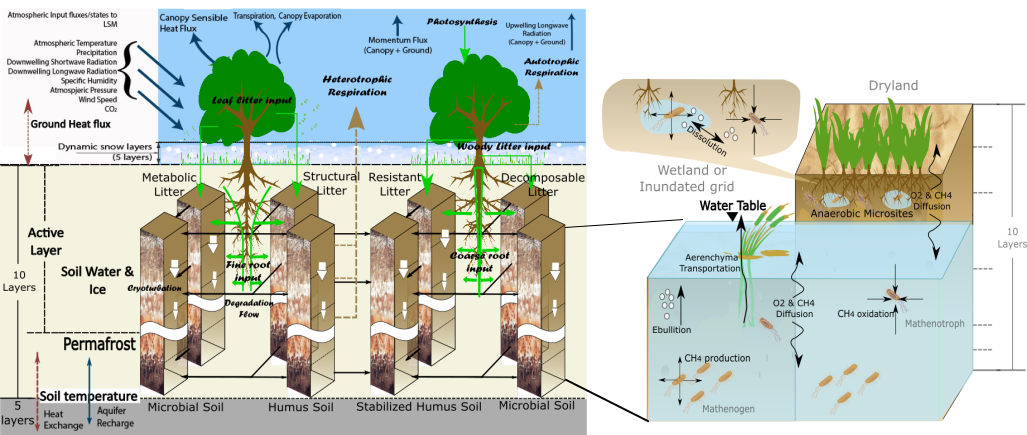
\includegraphics[width=0.9\columnwidth]{figures/ISAM_schematic_20161208.png}
 \caption{Schematic diagram of the ISAM model with the extended schemes.}
\end{figure}

\end{itemize}

\subsection*{Representation of Cryoturbation}

\begin{itemize}

 \item Cryoturbation is parameterized as the advective rate in the advection-diffusion equation describing vertical movement of SOC.
 \item The driver of cryoturbation is the growth of ice lens heaving nearby soil particles, which can be described by Miller's rigid ice lens growth model (O'Neill and Miller, 1985) derived from mass balance equation:
   \begin{equation}
   V_I=-k\frac{(\frac{\partial\psi_w}{\partial z}-\rho_wg)}{\rho_Ig(1-I_{pore})} 
   \end{equation}
   \begin{itemize}
     \item $V_I$ is the ice growth rate and also the ice lens growth velocity (mm/s)
     \item k is the hydraulic conductivity of the soil layer (mm/s)
     \item $\psi_w$ is the soil water potential of the corresponding layer (mm)
     \item $\rho_w$ and $\rho_I$ are constant water and ice density, respectively
     \item g is the gravitational acceleration ($kg/m^2$)
     and\\ 
     \item $I_{pore}$ is the fraction of pore ice in total soil ice
   \end{itemize}
   \item Ice lens is  separated from soil ice and initialized at the same time when start freezing and reset once the soil is completely thawed. We assume 50\% of the total soil ice to be initialized as ice lens.
 \item The linkage between frost heave rate and vertical cryoturbation rate is complicated by the soil structure and the plastic deformation modulus of soil particles. We simply generalize such a linkage through a decay parameter and the cryoturbation can be described as:
  \begin{equation}
  v=\frac{V_I}{\tau}
  \end{equation}
  \begin{itemize}
     \item v is the net vertical cryoturbation rate being coupled as the advective rate in the vertical soil movement model (mm/s)
     \item $\tau$ is the decay parameter and need to be calibrated
  \end{itemize}
\end{itemize}

%In this study, we used the F compset of the ACME model, in which the atmosphere and land models are active 
with the data ocean model and thermodynamic sea ice model. The atmosphere model is version 5 of the Community 
Atmosphere Model (CAM5) with the advanced spectral element dynamic core. In order to study the 
ENSO effects on the ecosystem, we activate the biogeochemistry component of the ACME land model. The sea surface
temperature (SST) and ice concentration are provided by the National Oceanic and Atmospheric Administration (NOAA) 
high resolution (1/4~$^{\circ}$) daily optimum Interpolation SST (OISST) for contemporary era. For future predictions, 
they are provided by the ensemble 9-month seasonal forecasts from NOAA Climate Forecast System (CFS) version 2 and 
the climatology reconstructed from historical observed SST. For simplicity, the horizontal grids of all ACME model 
components are the cubed sphere grid of ne30np4, approximately 1 by 1 degree.    
   


% \begin{figure}
%  \centering
%  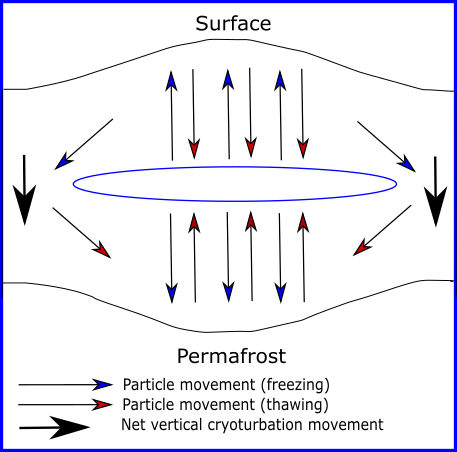
\includegraphics[width=0.47\columnwidth]{figures/Cryoturbation_scheme.png}
%  \caption{Schematic description of the cryotubation implemented in the model.}
% \end{figure}

\section*{Data and Experimental Design}
%%%%%%%%%%%%%%%%%%%%%%%%%%%%%%%%%%%%%%%%%%%%%%%%%%%%%%%%%%%%%%%%%%%%%%%%%%%%%%%
\subsection*{Data}
%\begin{tabular}{m{3cm} c}
% { As shown in Figure~\ref{fig:nee}, five Gelisol radiocarbon profiles (He et al., 2016) are selected to evaluate the modeled SOC storage and soil $\delta ^{14}C$ and determine the uncertain range of the decay parameter of cryoturbation rate $\tau$.} &
% 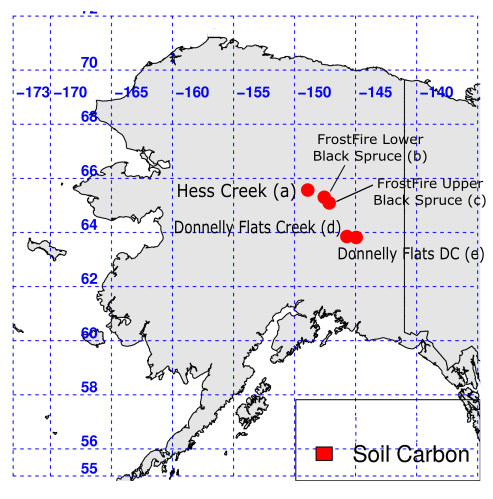
\includegraphics[width=0.65\columnwidth]{new_figures/Study_sites_annotated.png} \\
%   \caption{Location of the sites being used in this study.}\label{fig:nee}
%\end{tabular}

  \begin{itemize}
    \item As shown in Figure~\ref{fig:nee}, five Gelisol radiocarbon profiles (He et al., 2016) are selected to evaluate the modeled SOC storage and soil $\delta ^{14}C$ and determine the uncertain range of the decay parameter of cryoturbation rate $\tau$.
  \end{itemize}
\begin{figure}
   \centering
   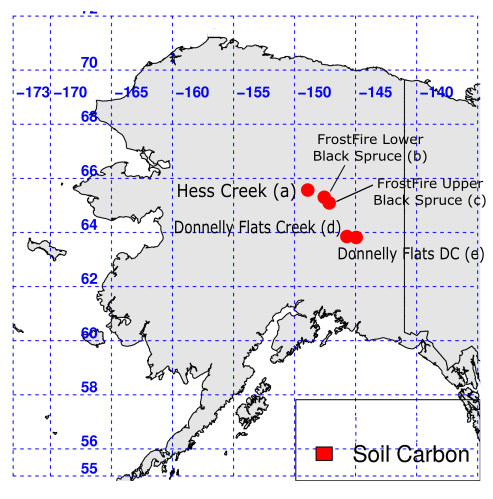
\includegraphics[width=0.5\columnwidth]{new_figures/Study_sites_annotated.png}
   \caption{Location of the sites being used in this study.}\label{fig:nee}
\end{figure}

%\begin{figure}
%\end{figure}

\subsection*{Experimental Design}
 \begin{itemize}
  \item ISAM-1DSCOC is set to perform single site spinup for the 5 radiocarbon sites (Figure 2) with all components (biogeophysics, gas diffusion, biogeochemistry and soil vertical movement) with fixed site specific land cover distribution. Soil texture, plant functional type and topographic factor for constraining lateral drainage were used to force the model. The spinup simulation cycled 1500 times with 1901 - 1920 CRU NCEP climate forcing due to the slow turnover of arctic SOC to reach the quasi-equilibrium of SOC storage.
  \item The historical simulation starts from 1801 till 2013 through forcing model with historical $CO_2$ concentration, N decomposition and atmospheric $\Delta ^{14}C$. In the first hundred years (1800-1899) we randomly pick climate forcing from 1901 to 1920. Starting year 1900 the historical climate forcing data is used.
  \item The decay parameter for determining cryoturbation rate is evaluated by matching the results of the historical run with observation sampled in the corresponding years.
  \item For each 14C site four cases of simulations under RCP8.5 scenario were performed from 2006 to 2100: (1) no cryoturbation, (2) using smallest decay parameter (i.e., highest sensitivity of cryoturbation to ice lens dynamics), (3) using calibrated decay parameter for each site, and (4) using largest decay parameter (i.e., lowest sensitivity of cryoturbation to ice lens dynamics). The projected SOC storage will be presented in the result section. The model is forced by the climate forcing data generated from the CESM1.2 RCP8.5 run.
% 
 \end{itemize}

\section*{Preliminary Results}
%%%%%%%%%%%%%%%%%%%%%%%%%%%%%%%%%%%%%%%%%%%%%%%%%%%%%%%%%%%%%%%%%%%%%%%%%%%%%%%

%\begin{itemize}
% \item The ACME v0.3 model was built and tested on Titan (OLCF), Cori and Edison (NERSC).
% \item The F-compset configuration was tested and performance optimized at both ne30 ($\sim$1$^\circ$) and ne120 ($\sim$$\frac{\textnormal{1}}{\textnormal{4}}$$^\circ$) resolutions. Given the queue wait times for moderately sized jobs and limited performance, we decided that ne120 was computationally prohibitive.
% \item The OISSTv2 data were remapped to the target ne30 grid to reduce the computational cost of remapping by the data ocean model at run time.
% \item The spin up simulation cycled 13 times (169 years), yielding a 10-y average NEE of $\sim$0~Pg\,C\,y$^{-\textnormal{1}}$ and an absolute value of NEE of $\sim$2~Pg\,C\,y$^{-\textnormal{1}}$
% \item A 25 year transient simulation through 2020 was performed and is analyzed below
%% \item Land model results are being valuated using the International Land Model Benchmarking (ILAMB) package, developed by the DOE-funded Biogeochemistry--Climate Feedbacks Scientific Focus Area project.
%
%\end{itemize}

% \subsection*{Water Table Evaluation}
% 
% As shown in Figure~\ref{fig:nee}, model correctly estimated the trend of water table varaiation, but still lacks enough representation for the small variation of water table in sites with a shallow water table (e.g., US-Bes site). This variation relates to a variable specific yield of different composition of organic layers (sapric, hemic and fibric) at top soil. 
% 
% \begin{figure}
%  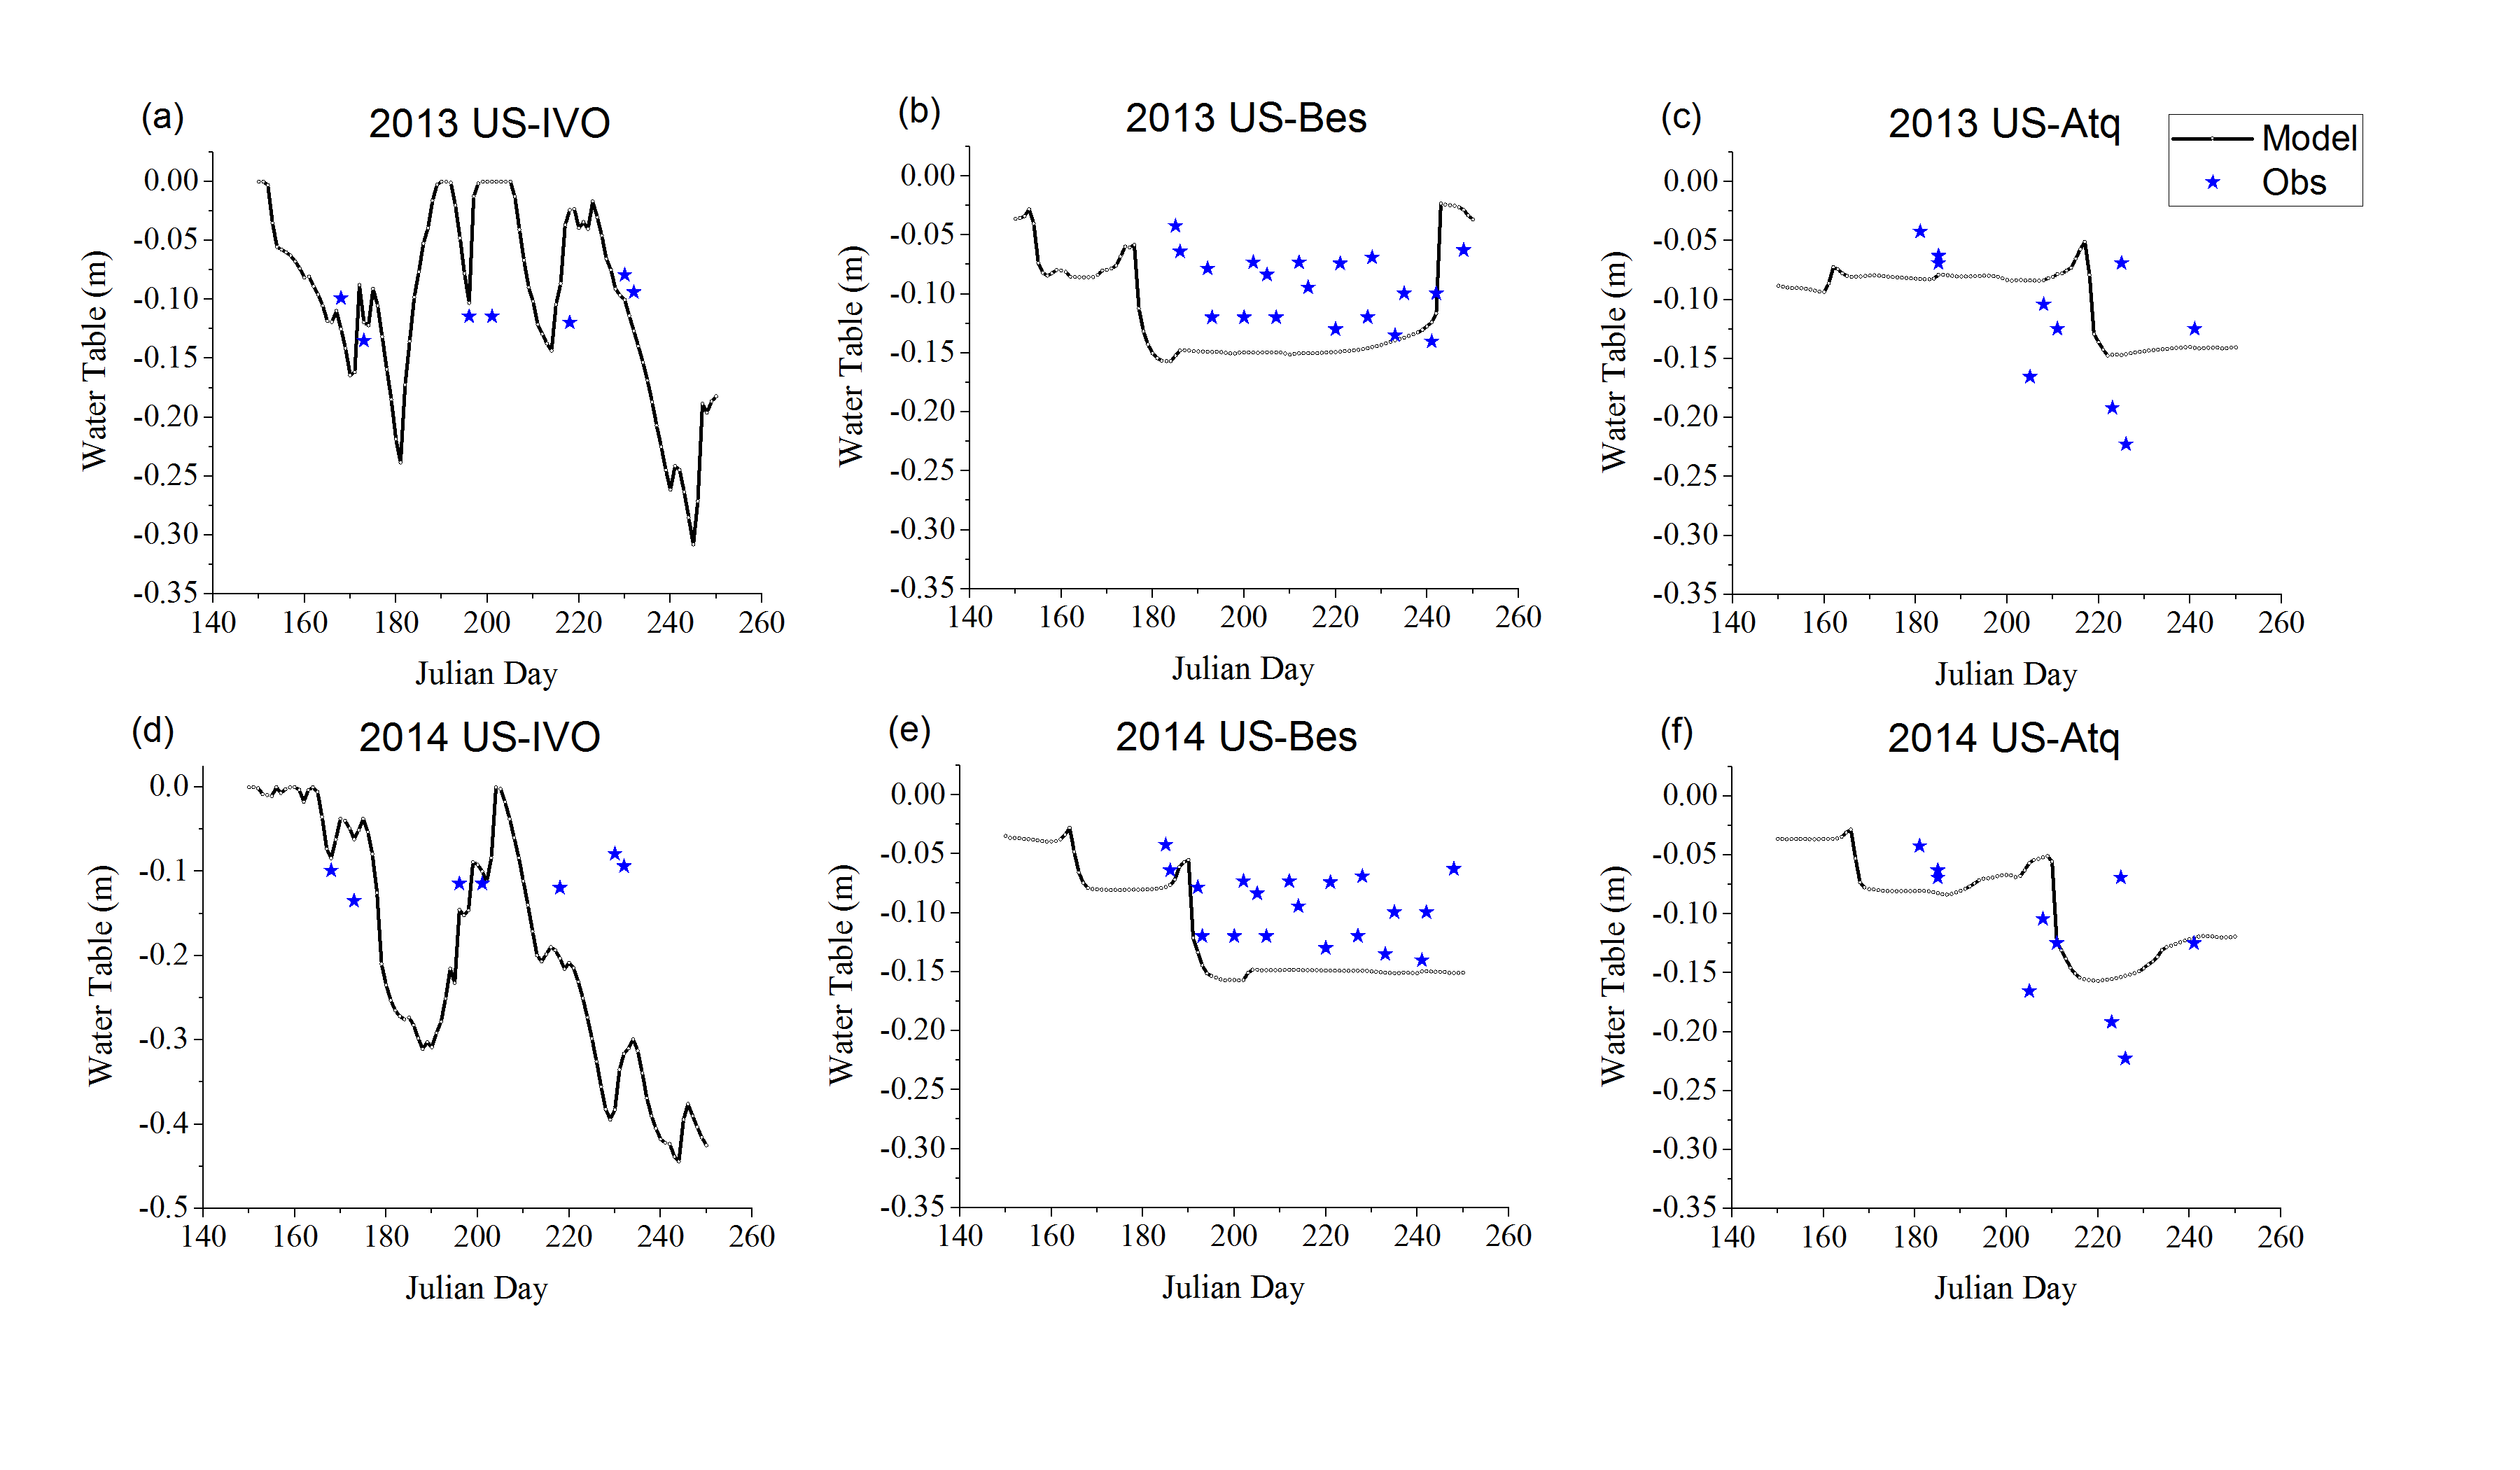
\includegraphics[width=0.9\columnwidth]{figures/Water_table.png}
%  \caption{The plot shows the comparison between observed and model simulated water table depth at three different sites. Three sites were forced by CRU-NCEP climate data from 1901 - 1920 and then perform the historical run with varying $CO_2$ and N deposition.}\label{fig:nee}
% \end{figure}

%\begin{figure}
% \begin{tabular}{c c}
%  \includegraphics[width=0.47\columnwidth]{figures/nee_10y_map1.png} &
%  \includegraphics[width=0.47\columnwidth]{figures/nee_10y_map2.png} \\
%  \includegraphics[width=0.47\columnwidth]{figures/nee_10y_map3.png} &
%  {\includegraphics[width=0.40\columnwidth]{figures/nee_plot.png}} \\
%  \includegraphics[width=0.47\columnwidth]{figures/nee_10y_colorbar.png} & \\ [-0.5em]
%  {\tiny g\,C\,m$^{-\textnormal{2}}$\,y$^{-\textnormal{1}}$} & \\
% \end{tabular}
% \caption{The maps show the 10-y mean net ecosystem exchange (NEE) from the spin up simulation for the a) first, b) second, and c) third decades of cycling the 1982--1994 OISSTv2 forcing. The plot in d) shows the global and tropical annual NEE (solid lines) and their five-year running averages (dashed lines) for the first 26 years of the spin up simulation.}\label{fig:nee}
%\end{figure}

%\subsection*{Climate Evaluation}
%
%\begin{figure}
% \begin{tabular}{c c}
%  CRU Mean Surface Air Temperature & Model Mean Surface Air Temperature \\
%  \includegraphics[trim=1.5cm 0cm 1.5cm 0cm,clip=true,width=0.48\columnwidth]{figures/temp_benchmark_global_timeint.png} &
%  \includegraphics[trim=1.5cm 0cm 1.5cm 0cm,clip=true,width=0.48\columnwidth]{figures/temp_acmev0.3enso_global_timeint.png} \\
%  \multicolumn{2}{c}{\includegraphics[width=0.60\columnwidth]{figures/temp_legend_timeint.png}} \\
%  Mean Surface Air Temperature Bias & Mean Annual Cycle \\
%  \includegraphics[trim=1.5cm 0cm 1.5cm 0cm,clip=true,width=0.48\columnwidth]{figures/temp_acmev0.3enso_global_bias.png} &
%  \includegraphics[width=0.48\columnwidth]{figures/temp_acmev0.3enso_global_cycle.png} \\
%  \includegraphics[trim=1.5cm 0cm 1.5cm 0cm,clip=true,width=0.48\columnwidth]{figures/temp_legend_bias.png} &
%  %\includegraphics[trim=0.9cm 5.2cm 8.2cm 0.8cm,clip=true,width=0.33\columnwidth]{figures/temp_legend_compcycle.png} \\
%  % But put some bottom margin back to shift the smaller version up a bit
%  \includegraphics[trim=0.9cm 4.5cm 8.2cm 0.8cm,clip=true,width=0.33\columnwidth]{figures/temp_legend_compcycle.png} \\
% \end{tabular}
% \caption{The ILAMB comparison of mean surface air temperature with the Climate Research Unit (CRU) benchmark shows the model captures the correct spatial pattern and annual cycle, but it exhibits about a +0.5~K global bias.}\label{fig:temp}
%\end{figure}
%
%\begin{figure}
% \begin{tabular}{c c}
%  GPCP2 Mean Precipitation & Model Mean Precipitation \\
%  \includegraphics[trim=1.5cm 0cm 1.5cm 0cm,clip=true,width=0.48\columnwidth]{figures/precip_benchmark_global_timeint.png} &
%  \includegraphics[trim=1.5cm 0cm 1.5cm 0cm,clip=true,width=0.48\columnwidth]{figures/precip_acmev0.3enso_global_timeint.png} \\
%  \multicolumn{2}{c}{\includegraphics[width=0.60\columnwidth]{figures/precip_legend_timeint.png}} \\
%  Mean Precipitation Bias & Mean Annual Cycle \\
%  \includegraphics[trim=1.5cm 0cm 1.5cm 0cm,clip=true,width=0.48\columnwidth]{figures/precip_acmev0.3enso_global_bias.png} &
%  \includegraphics[width=0.48\columnwidth]{figures/precip_acmev0.3enso_global_cycle.png} \\
%  \includegraphics[trim=1.5cm 0cm 1.5cm 0cm,clip=true,width=0.48\columnwidth]{figures/precip_legend_bias.png} &
%  %\includegraphics[trim=0.9cm 5.2cm 8.2cm 0.8cm,clip=true,width=0.33\columnwidth]{figures/precip_legend_compcycle.png} \\
  % But put some bottom margin back to shift the smaller version up a bit
%  \includegraphics[trim=0.9cm 4.5cm 8.2cm 0.8cm,clip=true,width=0.33\columnwidth]{figures/precip_legend_compcycle.png} \\
% \end{tabular}
% \caption{The ILAMB comparison of mean precipitation with the Global Precipitation Climatology Project version 2 (GPCP2) benchmark shows the model captures the correct spatial pattern, but it has reduced variability and exhibits a positive bias in high elevation regions.}\label{fig:precip}
%\end{figure}

\subsection*{SOC Storage of Historical Run}
\begin{itemize}
  \item Comparison shows the model is able to capture the trends of the SOC storage profiles collected at various NHL sites
  \item Soil samples sites for shrub lands (Figures b and c) have accumulated soil carbon of 7.75 and 7.76 $kgC/m^2$ that are relatively lower than other sites (20.35, 25.89 and 28.66 $kgC/m^2$, respectively) due to a strong CO2 fertilization effect and higher turnover of aboveground shrub comparing to boreal forest.
\end{itemize}

\begin{figure}
 \centering
 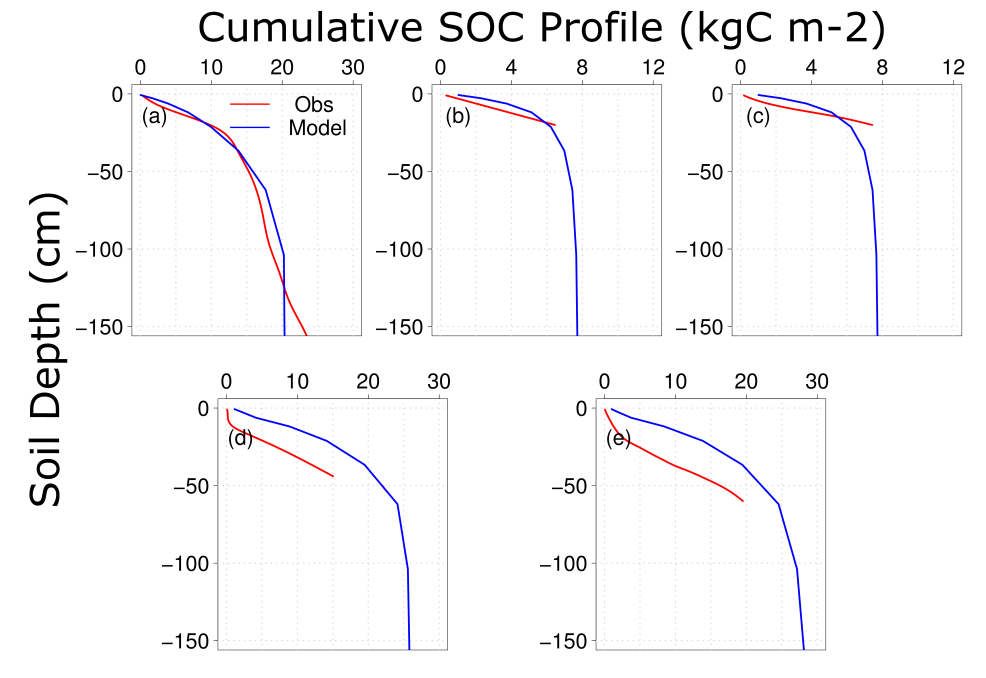
\includegraphics[width=0.9\columnwidth]{new_figures/Historical_SOC.png}
 \caption{Comparison of the model estimated cumulative depth distribution of SOC storage with soil sample data for (a) Hess Creek, (b) Frost-Fire Lower Black Spruce, (c) Frost-Fire Upper Balck Spruce, (d) Donnelly Flats Creek and (e) Donnelly Flat DC.}\label{fig:soc_hist}
\end{figure}

\subsection*{Radiocarbon Profile}
\begin{itemize}
  \item We implemented an isotopic carbon tracer into ISAM-1DSOC and forced the tracer by the atmospheric $\Delta ^{14}C$ compiled from several published studies (Levin and Kromer, 2004; Quan et al., 2013) and calibrated the decay parameter $\tau$ (shown for each site).
  \item The simulated soil $\Delta ^{14}C$ from model displays a good match to the general shape of the observed profiles while model tends to estimate a smaller or shallower peak $\Delta ^{14}C$ comparing to observation. 
  \item Figure 4(f) shows a set of sensitivity test for site (c) and indicated an overestimation of SOC turnover at the top soil that cannot be adjusted by tuning $\tau$ .
\end{itemize}

\begin{figure}
 \centering
 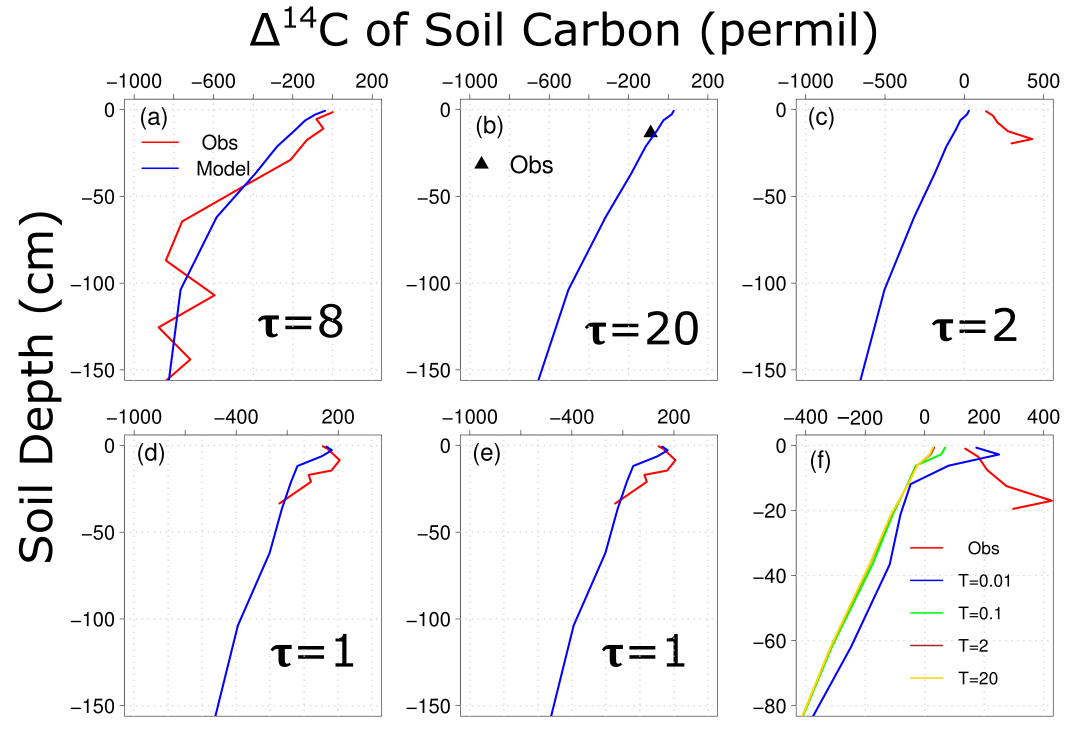
\includegraphics[width=0.9\columnwidth]{new_figures/Soil_D14_historical.png}
 \caption{Comparison of modeled and measured Soil $\Delta ^{14}C$ profiles. Subplot (f) shows the model outputs from a series of sensitivity experiments for site (c) by varying the decay parameter.}\label{fig:2014-2016_ENSO}
\end{figure}

\subsection*{Projected SOC storage under RCP8.5 Scenario}
\begin{itemize}
  \item We use $\tau$ = 1 as the low decay parameter and $\tau$ = 20 as the high decay parameter. 
  \item The change of SOC storage appears to be inconsistent between different sites, with three sites losing soil carbon but sites (b) and (c) gaining a total amount of 2 $kgC/m^2$ from 2006 to 2100 which mostly due to the strong $CO_2$ fertillizer effect and the fast turnover speed of shrub. 
  \item The no cryoturbation case (black line) estimates less multi-site mean SOC storgae comparing to the calibrated (red line, 0.15 $kgC/m^2$) and high (blue line, 0.09 $kgC/m^2$) cryoturbation cases and approximately the same SOC storage comapring to the low cryoturbation case. 
  \item The effect of cryoturbation on preserving carbon is strongly depend on speciic site, with site (a) shows 0.4 $kgC/m^2$ difference but only 0.12 $kgC/m^2$ for site (e). For site (a) the magnitude of the preservation effect is even higher than the total amount of the change of SOC storage (0.27 $kgC/m^2$ under no cryoturbation case).
\end{itemize}

\begin{figure}
 \centering
 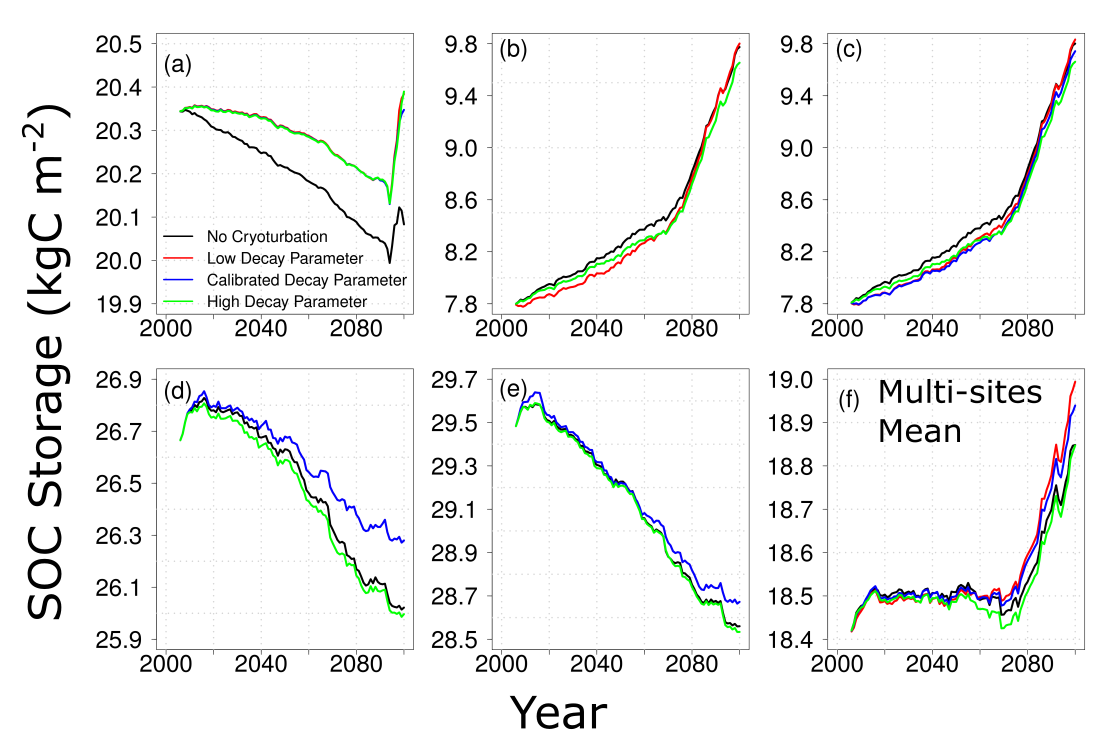
\includegraphics[width=0.9\columnwidth]{new_figures/Soil_SOC_RCP85projection.png}
 \caption{The projection of SOC storage at each site from 2006 - 2100.}\label{fig:2005_drought} 
\end{figure}

%%%%%%%%%%%%%%%%%%%%%%%%%%%%%%%%%%%%%%%%%%%%%%%%%%%%%%%%%%%%%%%%%%%%%%%%%%%%%%%
%\section*{Conclusions}
%%%%%%%%%%%%%%%%%%%%%%%%%%%%%%%%%%%%%%%%%%%%%%%%%%%%%%%%%%%%%%%%%%%%%%%%%%%%%%%

\vskip-0.25in
%%%%%%%%%%%%%%%%%%%%%%%%%%%%%%%%%%%%%%%%%%%%%%%%%%%%%%%%%%%%%%%%%%%%%%%%%%%%%%%
\section*{Summary and Next Steps}
%%%%%%%%%%%%%%%%%%%%%%%%%%%%%%%%%%%%%%%%%%%%%%%%%%%%%%%%%%%%%%%%%%%%%%%%%%%%%%%

\begin{itemize}
 %\item A set of ENSO simulation experiments have been defined and the spin up run is making progress on Titan.
 \item Evaluation of the historical simulation indicates that ISAM-1DSOC is able to reproduce the water table, SOC content profile and its vertical movement after the decay parameters being tuned to capture the site level condition
 \item Results of the soil $Delta ^{14}C$ profile indicate that the decay parameter could vary from 1.0 to 20.0, suggesting a wide range of the cryoturbation rate across the arctic region.
 \item Sites with peak $\Delta ^{14}C$ residing in subsoil can be caused by either the misrepresentation of SOC decomposition or missing processes other than cryoturbation (i.e. the vertical movement caused by freezing and thawing), possible mechanisms including strong bioturbation, the vertical deposition and the lateral transport of dissolved organic carbon.
 \item The projected SOC storage shows the importance of accounting for the potential damping of cryoturbation to soil carbon loss under RCP 8.5 projection. These results suggests that for global scale the decay parameter could vary with different soil groups.
 \item A full understanding on the implication of cryoturbation to the climate - carbon cycle feedback is needed for the next step.
\end{itemize}

%%%%%%%%%%%%%%%%%%%%%%%%%%%%%%%%%%%%%%%%%%%%%%%%%%%%%%%%%%%%%%%%%%%%%%%%%%%%%%%
%\begin{itemize}
%\item Blah
%
%\end{itemize}
%%%%%%%%%%%%%%%%%%%%%%%%%%%%%%%%%%%%%%%%%%%%%%%%%%%%%%%%%%%%%%%%%%%%%%%%%%%%%%%

%%%%%%%%%%%%%%%%%%%%%%%%%%%%%%%%%%%%%%%%%%%%%%%%%%%%%%%%%%%%%%%%%%%%%%%%%%%%%%%
%\section*{References}
%%%%%%%%%%%%%%%%%%%%%%%%%%%%%%%%%%%%%%%%%%%%%%%%%%%%%%%%%%%%%%%%%%%%%%%%%%%%%%%

%{
%\nocite{Hoffman_LandscapeEcol_20131001}
% \footnotesize%\rm
% \bibliographystyle{abbrvnat}
% \bibliography{refs/abbrev,%
%refs/Hargrove_EnvironManage_20040401,%
%refs/Hoffman_PDPTA99_19990628,%
%refs/Hoffman_LandscapeEcol_20131001,%
%refs/Walsh_JClim_20081201%
%%refs/Hoffman_MS-UTK-Physics_20041104,%
%%refs/White_GRL_20050218,%
%refs/Hargrove_JGS_20060701%
%}
%}

%\vskip-0.25in
%%%%%%%%%%%%%%%%%%%%%%%%%%%%%%%%%%%%%%%%%%%%%%%%%%%%%%%%%%%%%%%%%%%%%%%%%%%%%%%
\section*{References}
%%%%%%%%%%%%%%%%%%%%%%%%%%%%%%%%%%%%%%%%%%%%%%%%%%%%%%%%%%%%%%%%%%%%%%%%%%%%%%%

1. Ping, C.L., et al. Permafrost soils and carbon cycling. \textit{Soil}, 1.1 (2015): 147.\\
2. Barman, Rahul, and Atul K. Jain. Comparison of effects of cold region soil/snow processes and the uncertainties from model forcing data on permafrost physical characteristics. \textit{Journal of Advances in Modeling Earth Systems} 8.1, (2016).\\
3. Shu, Shijie, et al. Interactions Between Soil Organic Carbon Concentration and Soil Thermal and Hydraulic Dynamics and Its Impact on Soil Carbon Storage in Northern Highlatitudes. \textit{AGU Fall Meeting Abstracts} Vol. 1. (2015).\\
4. Swenson, S.C., et al. Improved simulation of the terrestrial hydrological cycle in permafrost regions by the Community Land Model. \textit{Journal of Advances in Modeling Earth Systems} 4.3 (2012).\\
5. O'Neill, Kevin, and Robert D. Miller. Exploration of a rigid ice model of frost heave. \textit{Water Resources Research} 21.3 (1985): 281-296.\\
%Zona, Donatella. et al. Cold season emissions dominate the Arctic tundra methane budget. \textit{Proceedings of the National Academy of Sciences} 113.1 (2016): 40-45.\\
6. He, Yujie et al. Radiocarbon constraints imply reduced carbon uptake by soils during the 21st century. \textit{Science} 353.6306 (2016): 1419-1424.\\
7. Levin, Ingeborg, and Bernd Kromer. The tropospheric 14CO2 level in mid latitudes of the northern hemisphere (1959-2003). \textit{Radiocarbon} 46.3 (2004): 1261-1271.\\
8. Hua, Quan, Mike Barbetti, and Andrzej Z. Rakowski. Atmospheric radiocarbon for the period 1950?2010. \textit{Radiocarbon} 55.4 (2013): 2059-2072.\\

%\vskip-0.25in
%%%%%%%%%%%%%%%%%%%%%%%%%%%%%%%%%%%%%%%%%%%%%%%%%%%%%%%%%%%%%%%%%%%%%%%%%%%%%%%
\section*{Acknowledgments}
%%%%%%%%%%%%%%%%%%%%%%%%%%%%%%%%%%%%%%%%%%%%%%%%%%%%%%%%%%%%%%%%%%%%%%%%%%%%%%%

%%%%%%%%%%%%%%%%%%%%%%%%%%%%%%%%%%%%%%%%%%%%%%%%%%%%%%%%%%%%%%%%%%%%%%%%%%%%%%%
%  \hfil
%  %
\includegraphics[height=1.5in,trim=1cm 1cm 1cm 1cm,clip=true]{logos/ACME_Logo.pdf}
%%  \includegraphics[height=1.5in]{logos/TES_logo-color_med.jpg}
%  \hspace*{1.5in}
%  %\hfil
%%  \includegraphics[height=1.5in]{logos/DOE_Office_of_Science_logo.pdf}
%  %\hfil
%  %\includegraphics[height=1.5in]{logos/USFS_Logo.png}
%  \hfil \\

\smallskip
\vbox{\small
This research was supported by the Office of Biological and Environmental 
Research in the U.S. Department of Energy Office of Science. }

%%%%%%%%%%%%%%%%%%%%%%%%%%%%%%%%%%%%%%%%%%%%%%%%%%%%%%%%%%%%%%%%%%%%%%%%%%%%%%%

\vfill
%%%%%%%%%%%%%%%%%%%%%%%%%%%%%%%%%%%%%%%%%%%%%%%%%%%%%%%%%%%%%%%%%%%%%%%%%%%%%%%
% \begin{minipage}[c]{\columnwidth}
% \begin{minipage}[c]{0.84\columnwidth}
%  \centering\Large\color{CCSIGreen}
%  \textbf{Want a copy of this poster to read later? \\ Scan this QR code with your smartphone!}
% \end{minipage}
% \begin{minipage}[c]{0.10\columnwidth}
%   \centering
%   \includegraphics[height=2.00in]{qrcode.36791219.png}
% \end{minipage}
% \end{minipage}

%%%%%%%%%%%%%%%%%%%%%%%%%%%%%%%%%%%%%%%%%%%%%%%%%%%%%%%%%%%%%%%%%%%%%%%%%%%%%%%

\end{multicols*}
\end{document} 
